\documentclass{memoir}
\usepackage{hyperref}
\usepackage{graphicx}
\graphicspath{ {figures/} }

\title{Distributed Systems:\\Crossing Intersection with Autonomous Vehicles}

\author{Antonio Toncetti\\Gabriele Venturato\\\\DMIF, University of Udine, Italy}

\date{%Version 0.1, 
	\today}

\begin{document}


%\begin{titlingpage}
\maketitle
\begin{abstract}
The aim of this project is to provide an implemented solution for the problem of crossing an intersection by autonomous vehicles.
Although it relies on some simplifications, this can be considered a real-case scenario for this problem.

The solution proposed here try to be more general and modular as possible, in order to be possibly extended in a concrete situation.
\end{abstract}
%\end{titlingpage}

\chapter{Introduction}\label{ch:intro}

The problem to solve is the one in which there is a crossroads, and some autonomous vehicles have to cross it without car accidents. 

The idea is to solve the problem for a generic intersection. The autonomous vehicles can't rely on a central server, they have to cooperate with each other to cross the intersection taking decisions that ensures a \emph{fair} and \emph{safe} policy. In particular there will be two actors in the proposed solution: vehicles and an environment. The latter is necessary in this context to simulate sensors that are usually inside an autonomous vehicle and that let it to move in the environment (e.g. GPS, cameras, etc\dots).
The system is \emph{fault tolerant}, but not byzantines processes nor cybersecurity are taken in consideration, for simplification purpose.

The report starts analyzing the project: Chapter~\ref{ch:analysis} is devoted to functional and non-functional requirements, and assumptions too. Chapter~\ref{ch:project} contains the description of the general architectures, and specific algorithms.

Then follows chapters aimed to: describe details of the implementation, and validation w.r.t. requirements.



\chapter{Analysis}\label{ch:analysis}

In this chapter are described in detail some fundamental assumptions, as well as functional and non-functional requirements.

\section{Assumptions}
Some general considerations are here presented. First of all it's assumed a situation in which each autonomous vehicle knows its destination and the roads it has to travel, since it's supposed to have a navigation system that allows this.

Moreover it's assumed, for sake of simplicity, that all vehicles have the same dimension --- or better: that each vehicle can fit into a single position of the internal model used to represent the roads.

Further assumptions are:

\begin{itemize}
	\item \emph{Faults}: at each moment a fault can happen in vehicles --- software or hardware. An hardware crash doesn't compromise the software abilities, but a software crash implies an hardware crash. Since we can assume that if the software fails, the hardware goes in ``emergency mode'' and stop itself. It's also assumed that if a crash happens in queues, there's enough space for the other vehicles to overtake the faulted one; but if the crash happen inside the crossroads it must be managed with the removal of the faulted vehicle by a tow truck (or something similar).
	\item \emph{Moves}: the path that a vehicle can take inside the interception is predefined and known a priori. From each position there's a unique path to each of the destinations, and no one can modify or choose a different path. An visual representation of this assumption can be found in Figure~\ref{fig:intersection-graph}, in which green dots represent position occupied while crossing, and light-blue dots are the destinations. Once a vehicle reaches its destination, it is considered ``satisfied'', and can not fail anymore, it can only move forward on its own way. Reverse is not allowed.
\end{itemize}

\begin{figure}
	\centering
	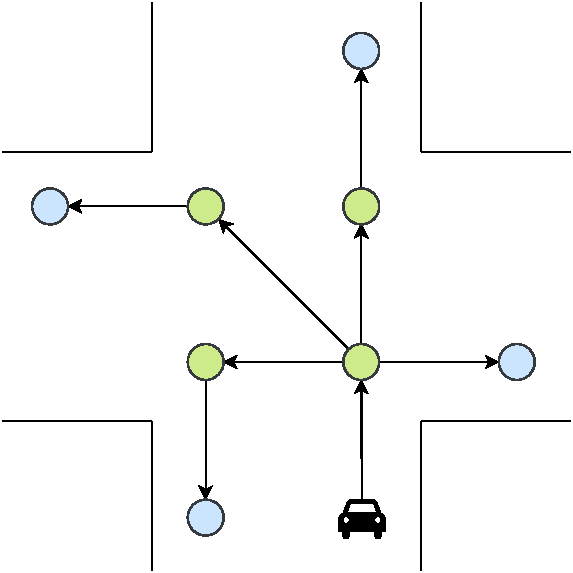
\includegraphics[width=0.4\linewidth]{intersection_graph.pdf}
	\caption{Example of predefined movements that a vehicle can follow in crossing an intersection.}
	\label{fig:intersection-graph}
\end{figure}

\section{Functional requirements}
The solution provide two main modules: \emph{vehicle} and \emph{environment}

\subsection{Vehicle}
Each vehicle at any moment has an internal state, and moreover:

\begin{itemize}
	\item knows its position and what happens around itself, through the environment (in a real context this is handled by sensors like GPS): it can view if there are other vehicles trying to cross, or if there are someone before or after its position;
	\item communicate with its neighbors sharing: the direction it want to travel, its internal state, its next position if allowed to move;
	\item if in the queue, it knows nothing but its internal information and that it is inside the queue with someone before it and possibly someone following, it can communicate only with these two;
	\item if in the first position of the queue, it can connect with the other vehicles that are going to cross (that are in the first position of the other queues), and to the vehicle behind it;
\end{itemize}

\subsection{Environment}
The environment represent vehicles possibility to use their sensors. It knows the intersection shape and dimension; it knows vehicles approaching the crossroads and the ones in the queues; it provide vehicles with all environmental information.

\section{Non functional requirements}
The system doesn't handle byzantines processes nor cybersecurity issues.

\begin{itemize}
	\item \emph{Safeness}: there can't be more than a vehicle in the same position at the same time;
	\item \emph{Liveness}: if a vehicle approaches the intersection and is waiting to cross it, eventually it will cross it;
	\item \emph{Fairness}: if a vehicle approaches the intersection and is waiting to cross it, there exists a bound for the waiting;
	\item \emph{Fault Tolerant}: the system is tolerant to hardware and software crashes;
	\item \emph{Distributed}: there is no central server, vehicles have to coordinate each other.
\end{itemize}



\chapter{Project}\label{ch:project}

The project is developed in \href{https://www.erlang.org/}{Erlang}

\section{Logical architecture}

\section{Protocols and algorithms}

\section{Physical architecture and deployment}

\section{Development plan}



%\chapter{Implementation}


%\chapter{Validation}


%\chapter{Conclusions}



%\appendix

%\chapter{Appendix}

\end{document}